%%  export TEXINPUTS=.:/home/mjw/src/manuals/common:

\documentclass[11pt,a4paper,openany,oneside]{book}

\usepackage[usenames]{color}
\usepackage{fancyhdr}
\usepackage{listings}
\usepackage{graphicx}
\usepackage{parskip}
\usepackage{enumitem}
\usepackage{latexsym}
\usepackage{titlesec}
\usepackage{xcolor}
\usepackage{hyperref} % wants to be last

\hypersetup{
  colorlinks   = true, %Colours links instead of ugly boxes
  urlcolor     = blue, %Colour for external hyperlinks
  linkcolor    = blue, %Colour of internal links
  citecolor   = red %Colour of citations
}

\pagestyle{fancy}
\renewcommand{\chaptermark}[1]{\markboth{\thechapter.\ #1}{}} 
\fancyhead[LE,LO]{\slshape \leftmark}
\fancyhead[RE,RO]{}

% Define some colours
\definecolor{OTTPGreen}{rgb}{0,0.341,0}

% Set formats for each heading level

\titleformat{\chapter}
{}
{\Huge\bfseries\sffamily\color{OTTPGreen}  \thechapter .\space}
{0pt}
{\Huge\bfseries\sffamily\color{OTTPGreen}}

\titleformat*{\section}{\Large\bfseries\sffamily\color{OTTPGreen}}
\titleformat*{\subsection}{\large\bfseries\sffamily\color{OTTPGreen}}
\titleformat*{\subsubsection}{\normalsize\bfseries\sffamily\color{OTTPGreen}}

\newcommand{\ci}[1]{\hspace*{1cm} {\small\texttt{#1}}}
\newcommand{\cc}[1]{{\texttt{#1}}}
% Set bullet style
\renewcommand{\labelitemi}{$\Box$} 

\newenvironment{description*}%
  {\setlength{\parskip}{0pt}%
	 \begin{description}%
		\setlength{\topsep}{-12pt}%
		\setlength{\itemindent}{-12pt}%
    \setlength{\itemsep}{0pt}%
		\setlength{\itemsep}{0pt}}%
  {\end{description}}

\newenvironment{enumerate*}%
  {\begin{enumerate}%
		\setlength{\topsep}{-12pt}%
		\setlength{\itemindent}{-12pt}%
    \setlength{\itemsep}{0pt}%
		\setlength{\parindent}{0pt}}%
  {\end{enumerate}}
  
\begin{document}

\begin{titlepage}

\begin{center}
\centerline{
\includegraphics{figures/ottplogo.png}}
\end{center}

\vspace*{4cm} 

\begin{center}
{\Huge The Open Traceable Time Platform}
\end{center}

\vspace*{4cm} 

\begin{center}
{\Huge User Manual}
\end{center}

\vspace*{4cm}

\begin{center}
Version 1.0
\end{center}

\begin{center}
Copyright 2016 E. Louis Marais, Michael Wouters
\end{center}

\end{titlepage}


\begin{titlepage}

\begin{center}
{\Large This work is licensed under a Creative \\
Commons Attribution 4.0 International License.}
\end{center}

\end{titlepage}

\tableofcontents
\listoffigures
\listoftables

\lstset{
	xleftmargin=24pt,
	basewidth=0.5em,
	basicstyle=\ttfamily,
	escapechar=\%
}

%% ****************************************************************************************
\chapter{Introduction}
%% ****************************************************************************************

\section{What is OpenTTP?}

\section{GPS common-view}

\section{The OpenTTP reference platform}

The OpenTTP reference platform consists of:
\begin{itemize}
\item BeagleBone Black
\item NVS NV08 GNSS receiver
\item Opal Kelly XEM6001 FPGA development board
\item Jackson Labs LTE Lite GPSDO
\item SSD
\item CrystalFontz LCD module
\end{itemize}

\section{Supported hardware}

	\subsection{GNSS receivers}
	
	\begin{table}
	\begin{tabular}{lll}
	Manufacturer & models & notes \\ \hline
	Javad & GRIL receivers & obsolete \\
	NVS   & NV08 & \\
	Trimble & Resolution T & obsolete\\
	ublox & Neo8MT & \\
	\end{tabular}
	\caption{Supported GPS/GNSS receivers.}
	\end{table}
	
	Note: OpenTTP uses a custom file format for logging GPS receiver data. It does not read native receiver binary-format files.
	
	Guidance on testing a receiver for suitability for time-transfer, and writing software to process
	the receiver's data, is given in the OpenTTP Developer's Guide.
	
	\subsection{Counter/timers}
	
	\begin{table}
	\begin{tabular}{lll}
	Manufacturer & models & notes \\ \hline
	Agilent & 5313x &  needs IOTech GPIB to RS232 converter\\
	OpenTTP &  & \\
	SRS & PRS10 & uses input 1 pps time-tagging function\\
	\end{tabular}
	\caption{Supported counter/timers.}
	\end{table}
	
%% ****************************************************************************************
\chapter{Getting started}
%% ****************************************************************************************

\section{Software installation requirements}

In addition to a basic Linux development environment, you will need the development packages for:
\begin{description*}
	\item[\cc{boost}]  C++ libraries
	\item[\cc{libgsl}] GNU scientific library
\end{description*}

Depending on your Linux installation, you may also need
\begin{description*}
	\item[\cc{Time::HiRes}] Perl library
\end{description*}

\section{Building and installing the software}

Two scripts are provided for installing the software.
\begin{lstlisting}
software/system/installsys.pl
software/gpscv/install.pl
\end{lstlisting}

\cc{installsys.pl} must be run first (with superuser privileges), 
because it installs libraries which are needed by the GPSCV software.

Run-time options can be viewed by running the script with the '-h' option. In particular, \cc{installsys.pl}
has options to list the available installation targets and to install particular targets.

\section{A minimal software setup}

Some users may only be interested in the core software that OpenTTP provides so that they can use
it with their own hardware. This section describes the minimum setup required for operation.

The OpenTTP software distribution is comprised of various C/C++ applications and Perl scripts.
As a minimum, you will need:
\begin{description*}
	\item \cc{TFLibrary.pm} Perl module for commonly used tasks, such as reading configuration files
	\item \cc{libconfigurator} C library for parsing configuration files
	\item \cc{lockport} utility to create a UUCP lock file
	\item \cc{mktimetx} creates time-transfer files
	\item one of the OpenTTP-provided scripts to log your receiver
	\item one of the OpenTTP-provided scripts to log your counter/timer
\end{description*}

You must use one of the OpenTTP receiver logging scripts for the GNSS receiver because \cc{mktimetx}
expects a custom file-format \ref{s:DataFileFormat}. In particular, the
receiver's native binary formats are not readable by \cc{mktimetx}. Similarly, OpenTTP uses a custom file
format for the counter-timer measurement files, although in this case, conversion from another format
will probably be straight-forward. Most likely, users will have to provide their own software for
logging their counter/timer, given the large number of possible devices here, and the limited
support within OpenTTP.

You may find the following useful:
\begin{description*}
	\item[] \cc{kickstart.pl} for automatic start of logging processes
	\item[] \cc{runmktimetx.pl} for automated processing, and reprocessing
	\item[] \cc{ziplogs.pl} for log file compression
\end{description*}	

Sample configuration files can be found in \cc{software/gpscv/common/etc}.
The user running the logging and processing needs the following directories (or equivalents - most paths
can be configured via the general configuration file, \ref{sgpscvconf}):
\cc{bin}, \cc{cggtts},\cc{etc},\cc{logs},\cc{raw},\cc{rinex},\cc{tmp}. Some of these paths can
be redefined in the configuration file \cc{gpscv.conf}.


%% ****************************************************************************************
\chapter{System hardware}
%% ****************************************************************************************


\begin{figure}
\centerline{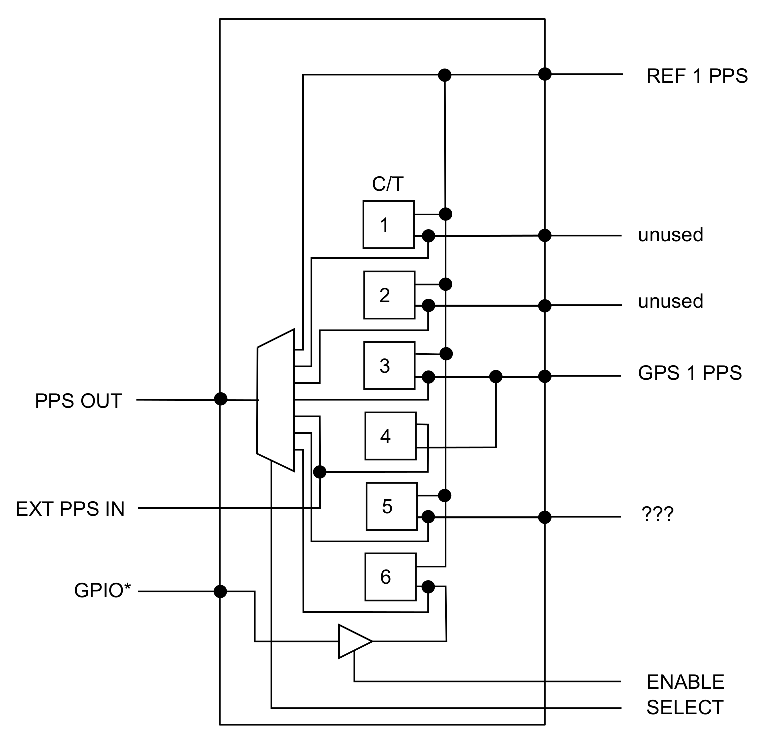
\includegraphics{figures/ottpcounter.eps}}
\end{figure}

\begin{table}
\begin{center}
\begin{tabular}{ll}
1 & channel 1 pps (unused)\\
2 & channel 2 pps (unused) \\
3 & channel 3 pps (GPS receiver)\\
4 & channel 4 pps (external pps)\\
5 & channel 5 pps (unused)\\
6 & channel 6 pps (GPIO)\\
7 & GPIO enabled\\
8 & Digital Clock Manager PLL is locked\\
\end{tabular}
\end{center}
\caption{Status LEDs}
\end{table}


%% ****************************************************************************************
\chapter{GPSCV software}
%% ****************************************************************************************

\section{Software overview}

\begin{table}[h]
\begin{tabular}{l|l|l}
	& program & \\ 
	\hline
GPSCV processing  &  & \\
	& \hyperlink{h:mktimetx}{mktimetx} & core program\\
	& \hyperlink{h:runmktimetx}{runmktimetx.pl} & \\
	\hline
TIC logging & & \\
	& \hyperlink{h:hp5313xlog}{hp5313xlog.pl} &\\
	& \hyperlink{h:okxemlog}{okxemlog.pl} & \\
	& \hyperlink{h:prs10log}{prs10log.pl} & \\
	\hline
GNSS receiver logging & & \\
	&	\hyperlink{h:jnslog}{jnslog.pl} & Javad\\
	& \hyperlink{h:nvslog}{nvslog.pl} & NVS\\
	& \hyperlink{h:restlog}{restlog.pl} & Trimble Resolution T\\
	& \hyperlink{h:ubloxlog}{ubloxlog.pl} & ublox\\
GNSS receiver utilities & & \\
	& \hyperlink{h:restextract}{restextract.pl} & \\
	\hline
Analysis tools & & \\
	& \hyperlink{h:rxdelaycal}{rxdelaycal.pl} & \\
	\hline
\end{tabular}
\caption{GPSCV software overview}
\end{table}

\section{Configuration file format \label{sConfigFileFormat}}

Configuration files use a common format and are plain text files, designed to be easily edited via a command-line
editor because in many applications, only shell access to the system will be available.

The file is divided into sections, with section names delimited by square brackets [ ]. Entries in each section
are of the form:
\begin{lstlisting}
key = value
\end{lstlisting}
For example,
\begin{lstlisting}
[Receiver]
manufacturer = Trimble
model = Resolution T
\end{lstlisting}
defines a section \cc{Receiver} and the two keys: \cc{manufacturer} and \cc{model}. 

The notation \cc{Section::Key} is used to fully specify keys. For example,
\cc{Receiver::model} and \cc{Receiver::manufacturer} specify the two keys above.

Keys and section names are not case-sensitive. Comments begin with a `\#'.

Some keys define a list of sections. For example, the comma-separated list of values for \cc{CGGTTS::outputs} 
\begin{lstlisting}
[CGGTTS]
outputs = C1-code,P1-code,P2-code
\end{lstlisting}
defines three sections: \cc{C1-code}, \cc{P1-code}, and \cc{P2-code}.

\section{Data file formats \label{s:DataFileFormat}}

\subsection{GPS receiver}

This text file records messages from the GPS receiver. The messages can be a mix of ASCII and binary messages.
Binary messages are hexadecimal-encoded. Some logging scripts record ancillary information, 
such as commands sent to the receiver. Comments are allowed, prefaced by a `\#' character. 
The `@' character can be used to tag lines containing special information that needs to be parsed by
the processing software.

Messages are successive lines of the form:
\begin{lstlisting}
<message_id> <time_stamp> <message>
\end{lstlisting}
\textit{Example:}
\begin{lstlisting}
TO 00:00:02 cdfbc75a9a8c353fc5
\end{lstlisting}

Hex encoding of binary messages results in much larger files but these compress to a size not much larger
than the original binary data.

\subsection{Time-interval counter}

This text file records the difference between GNSS receiver and the Reference Oscillator 1 pps,
measured each second. Entries are successive lines of the form:
\begin{lstlisting}
<time_of_day> <time_difference>
\end{lstlisting}
where the time difference is in seconds.\\
\textit{Example:}
\begin{lstlisting}
00:00:04  +4.0821E-006 
\end{lstlisting}


\section{gpscv.conf - the core configuration file \label{sgpscvconf} }

A single configuration file, \cc{gpscv.conf}, provides configuration information to most of the
OpenTTP software. 
\cc{gpscv.conf} is used by \cc{mktimetx}, receiver logging scripts, TIC logging scripts,receiver utilities and so on.

It uses the format described in \ref{sConfigFileFormat}.

\begin{table}[ht]
\begin{tabular}{l|p{10cm}}
Section & Key \\ \hline
\hyperlink{h:antenna}{Antenna} & antenna number, antenna type, 
				delta H, delta N, delta E, frame,
				marker name, marker number,
				X, Y, Z\\ \hline
\hyperlink{h:cggtts}{CGGTTS} & BIPM cal id, comments, create, 
         ephemeris, ephemeris file, ephemeris path,
         internal delay, lab id, maximum DSG, minimum elevation,
         minimum track length, naming convention, outputs, reference,
         receiver id, revision date, version,
         code, constellation, path
         \\ \hline
\hyperlink{h:delays}{Delays}  & antenna cable, reference cable 
         \\ \hline
\hyperlink{h:counter}{Counter} & file extension, GPIB address, header generator, lock file,
         logger, logger options, okxem channel, port
				\\ \hline
\hyperlink{h:misc}{Misc}    & gzip
				\\ \hline
\hyperlink{h:paths}{Paths} & CGGTTS, counter data, processing log, receiver data, RINEX, tmp
				\\ \hline
\hyperlink{h:receiver}{Receiver} & configuration, elevation mask, logger, logger options, 
				 manufacturer, model, observations, 
         port, pps offset, synchronization, pps synchronization delay,
         status file, timeout, version
				\\ \hline
\hyperlink{h:reference}{Reference} & file extension, logging interval, log path, log status, oscillator, power flag, status file
        \\ \hline
\hyperlink{h:rinex}{RINEX}  & agency, create, observer, version
				\\ \hline
\end{tabular}
\caption{Summary of \cc{gpscv.conf} entries}
\end{table}

\subsection{[Antenna] section}

Entries used to create the RINEX header are:
\begin{itemize}
\item antenna number
\item antenna type
\item delta H, delta E, delta N
\item marker name
\item marker number
\item X,Y,Z
\end{itemize}

Entries used to create the CGGTTS header are:
\begin{itemize}
\item X,Y,Z
\end{itemize}

\hypertarget{h:antenna}{}
{\bfseries antenna number}\\
This appears as ANTNUM in the RINEX header.\\
\textit{Example:}
\begin{lstlisting}
antenna number = A567456
\end{lstlisting}

{\bfseries antenna type}\\
This appears as ANTTYPE in the RINEX header.\\
\textit{Example:}
\begin{lstlisting}
antenna type = Ashtec
\end{lstlisting}

{\bfseries delta H}\\
This appears as DELTA H in the RINEX header.\\
\textit{Example:}
\begin{lstlisting}
delta H = 0.0
\end{lstlisting}

{\bfseries delta E}\\
This appears as DELTA E in the RINEX header.\\
\textit{Example:}
\begin{lstlisting}
delta E = 0.0
\end{lstlisting}

{\bfseries delta N}\\
This appears as DELTA N in the RINEX header.\\
\textit{Example:}
\begin{lstlisting}
delta N = 0.0
\end{lstlisting}

{\bfseries frame}\\
This appears as FRAME in the CGGTTS header.\\
\textit{Example:}
\begin{lstlisting}
frame = ITRF2010
\end{lstlisting}

{\bfseries marker name}\\
This appears as MARKER NAME in the RINEX header.\\
\textit{Example:}
\begin{lstlisting}
marker name =
\end{lstlisting}

{\bfseries marker number}\\
This appears as MARKER NUMBER in the RINEX header.\\
\textit{Example:}
\begin{lstlisting}
marker number =
\end{lstlisting}

{\bfseries X}\\
This appears as X in the CGGTTS header and APPROX POSITION XYZ in the RINEXheader.\\
\textit{Example:}
\begin{lstlisting}
X = +4567890.123
\end{lstlisting}

{\bfseries Y}\\
This appears as Y in the CGGTTS header and APPROX POSITION XYZ in the RINEXheader.\\
\textit{Example:}
\begin{lstlisting}
Y = +2345678.90
\end{lstlisting}

{\bfseries Z}\\
This appears as Z in the CGGTTS header and APPROX POSITION XYZ in the RINEXheader.\\
\textit{Example:}
\begin{lstlisting}
Z = -1234567.890 
\end{lstlisting}


\subsection{[CGGTTS] section }

\hypertarget{h:cggtts}{Entries} in this section control the format and content of CGGTTS files 
and filtering applied to CGGTTS tracks in the final output.

To create CGGTTS output you must enable it: 


{\bfseries outputs}\\
This defines a list of sections which in turn define the desired CGGTTS outputs.\\
\textit{Example:}
\begin{lstlisting}
outputs = CGGTTS-GPS-C1,CGGTTS-GPS-P1,CGGTTS-GPS-P2
\end{lstlisting}

A CGGTTS v2E header looks like:
\begin{lstlisting}
CGGTTS     GENERIC DATA FORMAT VERSION = 2E
REV DATE = 2018-03-20
RCVR = NVS NV08 undefined 1999 mktimetx,v0.1.4
CH = 32
IMS = 99999
LAB = NMIA
X = -4648239.852 m
Y = +2560635.623 m
Z = -3526317.023 m
FRAME = ITRF2008
COMMENTS = none
INT DLY = 0.0 ns (GPS C1)     CAL_ID = none
CAB DLY = 0.0 ns
REF DLY = 0.0 ns
REF = UTC(AUS)
CKSUM = 1A
\end{lstlisting}

Entries in the header than can be defined in the CGGTTS section are as below. 

{\bfseries comments}\\
This defines a single COMMENTS line in the CGGTTS header.
The output line will be truncated at 128 characters.\\
\textit{Example:}
\begin{lstlisting}
comments = none
\end{lstlisting}

{\bfseries lab }\\
This defines the LAB line.\\
\textit{Example:}
\begin{lstlisting}
lab = NMI
\end{lstlisting}

{\bfseries reference}\\
This defines REF in the CGGTTS header.\\
\textit{Example:}
\begin{lstlisting}
reference = UTC(XXX)
\end{lstlisting}

{\bfseries revision date}\\
This defines REV DATE in the CGGTTS header. It must be in the format YYYY-MM-DD.\\
\textit{Example:}
\begin{lstlisting}
revision date = 2015-12-31
\end{lstlisting}


{\bfseries create}\\
This defines whether or not CGGTTS files will be generated by \cc{mktimetx}.\\
\textit{Example:}
\begin{lstlisting}
create = yes
\end{lstlisting}

{\bfseries ephemeris}\\
This defines whether to use the receiver-provided ephemeris or a user-provided ephemeris (via a RINEX navigation file).
If a user-provided ephemeris is specified then \cc{ephemeris path} and \cc{ephemeris file} 
must also be specified.\\
\textit{Example:}
\begin{lstlisting}
ephemeris = receiver
\end{lstlisting}

{\bfseries ephemeris file}\\
This specifies a pattern for user-provided RINEX navigation files.
Currently, only patterns of the form \cc{XXXXddd0.yyn} are recognized.\\
\textit{Example:}
\begin{lstlisting}
ephemeris file = brdcddd0.yyn
\end{lstlisting}

{\bfseries ephemeris path}\\
This specifies the path to user-provided RINEX navigation files.\\
\textit{Example:}
\begin{lstlisting}
ephemeris path = igsproducts
\end{lstlisting}

{\bfseries lab id}\\
This defines the two-character lab code used for creating BIPM-style file names, as per the V2E specification.\\
\textit{Example:}
\begin{lstlisting}
lab id = AU
\end{lstlisting}

{\bfseries maximum DSG}\\
CGGTTS tracks with DSG lower than this will be filtered out. 
The units are ns.\\
\textit{Example:}
\begin{lstlisting}
maximum DSG = 10.0
\end{lstlisting}

{\bfseries minimum elevation}\\
CGGTTS tracks with elevations lower than this will be filtered out. 
The units are degrees.\\
\textit{Example:}
\begin{lstlisting}
minimum elevation = 10
\end{lstlisting}

{\bfseries minimum track length}\\
CGGTTS tracks shorter than this will be filtered out. Tracks meeting the criterion are not necessarily contiguous.
The units are seconds.\\
\textit{Example:}
\begin{lstlisting}
minimum track length = 390
\end{lstlisting}

{\bfseries maximum URA}\\
GPS ephemerides with URA greater than this will not be used. 
They will still be written to RINEX navigation files, however.\\
\textit{Example:}
\begin{lstlisting}
maximum URA = 3.0
\end{lstlisting}

{\bfseries naming convention}\\
Defines the CGGTTS file naming convention. Valid options are `plain' (MJD.cctf) and `BIPM' styles.
The \cc{lab id} and \cc{receiver id} should be defined in conjunction with BIPM-style filenames.\\
\textit{Example:}
\begin{lstlisting}
naming convention = BIPM
\end{lstlisting}

{\bfseries receiver id}\\
This defines the two-character receiver code used for creating BIPM-style file names, 
as per the V2E specification.\\
\textit{Example:}
\begin{lstlisting}
receiver is = 01
\end{lstlisting}

{\bfseries version}\\
This defines the version of CGGTTS output. Valid versions are v1 and v2E. 
The \cc{lab id} and \cc{receiver id} should be defined in conjunction with v2E ouput\\
\textit{Example:}
\begin{lstlisting}
version = v2E
\end{lstlisting}


\subsubsection{CGGTTS output sections}

Multiple CGGTTS outputs can be defined, allowing for different constellation and signal combinations.
An example of a CGGTTS output section is as follows:
\begin{lstlisting}
[CGGTTS-GPS-C1]
constellation=GPS
code=C1
path=cggtts
BIPM cal id = none
internal delay = 11.0
\end{lstlisting}

{\bfseries BIPM cal id}\\
This defines CAL\_ID for the internal delay, as used in v2E CGGTTS headers.\\
\textit{Example:}
\begin{lstlisting}
BIPM cal id = none
\end{lstlisting}

{\bfseries code}\\

CGGTTS codes can be specified using either the two letter code, for example `C1' as described in the CGGTTS V2E 
specification, or three letter RINEX v3.03 observation codes.
\begin{table}
\begin{tabular}{ll}
	CGGTTS name	 & RINEX name \\ \hline
	C1 & C1C \\
	P1 & C1P \\
	E1 & C1C \\
	B1 & C2I \\
	C2 & C2C \\
	P2 & C2P \\
	B2 & C7I 
\end{tabular}
\caption{Correspondence of CGGTTS and RINEX signal names.}
\end{table}
\textit{Example:}
\begin{lstlisting}
code = P1+P3
\end{lstlisting}

{\bfseries constellation}\\
This defines the GNSS constellation. Only GPS is supported currently for CGGTTS generation.\\
\textit{Example:}
\begin{lstlisting}
constellation = GPS
\end{lstlisting}

{\bfseries internal delay}\\
This defines INT DLY in the CGGTTS header. The units are ns.\\
\textit{Example:}
\begin{lstlisting}
INT DLY = 0.0
\end{lstlisting}

{\bfseries path}\\
This defines the directory in which output files are placed.\\
\textit{Example:}
\begin{lstlisting}
path = cggtts
\end{lstlisting}

In v1 CGGTTS files, the delays are specified via INT DLY, CAB DLY and ANT DLY.  
For v2E files, the delays may be specified via the `system delay' and `total delay'.
If multiple delays (eg both internal and system delay are present) are defined in
\cc{gpscv.conf}, the precedence order is internal, system and then total delay.

The entries used to specify system and total delay are:\\

{\bfseries system delay}\\
This defines SYS DLY in the CGGTTS header. The units are ns.\\
\textit{Example:}
\begin{lstlisting}
SYS DLY = 0.0
\end{lstlisting}

{\bfseries total delay}\\
This defines TOT DLY in the CGGTTS header. The units are ns.\\
\textit{Example:}
\begin{lstlisting}
TOT DLY = 0.0
\end{lstlisting}

\subsection{[Counter] section}

\hypertarget{h:counter}{}

{\bfseries file extension}\\
This defines the extension used for time interval measurement files.
The default is `tic'.\\
\textit{Example:}
\begin{lstlisting}
file extension = tic
\end{lstlisting}

{\bfseries configuration}\\ \hypertarget{h:counter_configuration}{}
This sets a configuration file for the counter. Its contents are defined by the calling script.
In the case of HP5313x counters for example,
it lists SCPI commands sent to initiliaze the counter.\\
\textit{Example:}
\begin{lstlisting}
configuration = etc/hp53131.conf
\end{lstlisting}

{\bfseries flip sign}\\
The processing software eg \cc{mktimetx} assumes that TIC measurements are started by the reference
and stopped by the GNSS receiver. If you need to invert the sign of the measurements, set the option
`flip sign' to `yes',
\textit{Example:}
\begin{lstlisting}
flip sign = no 
\end{lstlisting}

{\bfseries GPIB address}\\ \hypertarget{h:counter_gpib_address}{}
For GPIB devices, the GPIB address must be defined.\\
\textit{Example:}
\begin{lstlisting}
GPIB address = 3
\end{lstlisting}

{\bfseries GPIB converter}\\  \hypertarget{h:counter_gpib_converter}{}
This defines the GPIB interface converter (eg RS232 to GPIB).
Currently the only valid values is `Micro488'.\\
\textit{Example:}
\begin{lstlisting}
GPIB converter = Micro488
\end{lstlisting}

{\bfseries header generator}\\
A header for the log file can be optionally added to the log file, using the output
of a user provided script. Output should be to \cc{stdout}.
Each line will have a ``\#'' automatically prepended to it.\\
\textit{Example:}
\begin{lstlisting}
header generator = bin/myticheader.pl
\end{lstlisting}

{\bfseries lock file}\\
This defines the device lock file, used to prevent multiple instances of the logger
from being started.\\
\textit{Example:}
\begin{lstlisting}
lockfile = okxem.gpscv.lock
\end{lstlisting}

{\bfseries logger}\\
This defines the counter logging script.\\
\textit{Example:}
\begin{lstlisting}
logger = okxemlog.pl
\end{lstlisting}

{\bfseries logger options}\\
This defines options passed to the counter logging script.\\
\textit{Example:}
\begin{lstlisting}
logger options =
\end{lstlisting}

{\bfseries mode}\\ \hypertarget{h:counter_mode}{}
This defines the operating mode of the counter.
Valid values are \cc{timestamp} and \cc{time interval}
Currently, this is only used by the TAPR TICC.\\
\textit{Example:}
\begin{lstlisting}
mode = timestamp
\end{lstlisting}

{\bfseries okxem channel}\\ \hypertarget{h:counter_okxem_channel}{}
The OpenTTP counter is multi-channel so the channel to use (1-6) must be specified.\\
\textit{Example:}
\begin{lstlisting}
okxem channel=3
\end{lstlisting}

{\bfseries port}\\ \hypertarget{h:counter_port}{}
This defines the port used to communicate with the counter. It's value depends on the type of counter. 
For the XEM6001, it's a Unix socket. For serial devices, it's a device name like
\cc{/dev/ttyUSB0}.\\
\textit{Example:}
\begin{lstlisting}
# this is the port used by okcounterd
port = 21577 
\end{lstlisting}

{\bfseries timestamp format}\\ \hypertarget{h:counter_timestamp_format}{}
This controls the format of timestamps used in the counter log file.
Valid values are \cc{unix} and \cc{time of day}.
Currently, this is only used by the TAPR TICC.\\
\textit{Example:}
\begin{lstlisting}
timestamp format = time of day
\end{lstlisting}

\subsection{[Misc] section}

\hypertarget{h:misc}{}

{\bfseries gzip}\\
Defines the compression/decompression program used in conjunction with counter and receiver log files.\\
\textit{Example:}
\begin{lstlisting}
gzip = /bin/gzip 
\end{lstlisting}

\subsection{[Delays] section}

\hypertarget{h:delays}{}

{\bfseries antenna cable}\\
This is ANT DLY as used in the CGGTTS header. Units are ns.\\
\textit{Example:}
\begin{lstlisting}
antenna cable = 0.0
\end{lstlisting}

{\bfseries reference cable}\\
This is REF DLY as used in the CGGTTS header. Units are ns.\\
\textit{Example:}
\begin{lstlisting}
reference cable = 0.0
\end{lstlisting}

\subsection{[Paths] section} 

\hypertarget{h:paths}{}

Paths follow the rules described in .

{\bfseries root}\\ \hypertarget{h:rootpath}{}
Defines the root path to be used with all other paths, unless they are specified as absolute paths.
As with other paths specified in \cc{gpscv.conf}, it is interpreted as being relative to the user's
home directory, unless prefaced with a `/'.\\
\textit{Example:}
\begin{lstlisting}
root = test/newreceiver
\end{lstlisting}

{\bfseries CGGTTS}\\
Defines the default directory used for CGGTTS files.
This is typically overridden by the output directory that can be  defined in each CGGGTS output section.\\
\textit{Example:}
\begin{lstlisting}
CGGTTS = cggtts
\end{lstlisting}

{\bfseries counter data}\\
Defines the directory used for TIC data files.\\
\textit{Example:}
\begin{lstlisting}
counter data = raw
\end{lstlisting}

{\bfseries processing log}\\
Defines the directory where the \cc{mktimetx} processing log is written.\\
\textit{Example:}
\begin{lstlisting}
processing log = logs
\end{lstlisting}

{\bfseries receiver data}\\
Defines the directory used for GNSS receiver raw data files.\\
\textit{Example:}
\begin{lstlisting}
receiver data = raw
\end{lstlisting}

{\bfseries RINEX}\\
Defines the directory used for RINEX files.\\
\textit{Example:}
\begin{lstlisting}
RINEX = rinex
\end{lstlisting}

{\bfseries tmp}\\
Defines the directory used for intermediate and debugging files.\\
\textit{Example:}
\begin{lstlisting}
tmp = tmp
\end{lstlisting}

{\bfseries onewire temp data}\\
Defines the directory used to write temperature logs.\\
\textit{Example:}
\begin{lstlisting}
onewiretemp data = raw/onewire
\end{lstlisting}

{\bfseries uucp lock}\\
Sets the directory used to write UUCP lock files. UUCP lock files are used with serial devices to prevent
other processes (eg \cc{minicom}) opening the serial port while it is in use. The default is \cc{/var/lock}
but this varies with the operating system and its version so you will need to check this.\\
\textit{Example:}
\begin{lstlisting}
# This is for Debian
uucp lock = /var/run/lock
\end{lstlisting}

{\bfseries rinex l1l2}\\ \hypertarget{h:rinex_l1l2}{}
Defines the directory used to write RINEX files with all observations, typically so that precise antenna coordinates
can be obtained. This is only used with dual frequency Javad receivers.\\
\textit{Example:}
\begin{lstlisting}
rinex l1l2 = rinex/l1l2
\end{lstlisting}


\subsection{[Receiver] section \label{sgcreceiver}}

\hypertarget{h:receiver}{}

{\bfseries configuration}\\
\\
\textit{Example:}
\begin{lstlisting}
configuration = etc/rx.conf
\end{lstlisting}

{\bfseries elevation mask}\\
This sets an elevation mask for tracking os satellites - below this elevation, satellites
are ignored. The units are degrees. This may not be implemented for all receivers.\\
\textit{Example:}
\begin{lstlisting}
elevation mask = 0
\end{lstlisting}

{\bfseries logger}\\
This is the script used to configure and log messages from the GNSS receiver.\\
\textit{Example:}
\begin{lstlisting}
logger = jnslog.pl
\end{lstlisting}

{\bfseries logger options}\\
These are options passed to the receiver logging script.\\
\textit{Example:}
\begin{lstlisting}
logger options =
\end{lstlisting}

{\bfseries manufacturer}\\
This defines the manufacturer of the receiver. Together with the model and version, 
this sets how data from the receiver is processed. For a list of supported receivers
see XX.\\
\textit{Example:}
\begin{lstlisting}
manufacturer = Javad
\end{lstlisting}

{\bfseries model}\\
This is the receiver model.For a list of supported receivers
see XX.\\
\textit{Example:}
\begin{lstlisting}
model = HE_GGD
\end{lstlisting}

{\bfseries version}\\
This can be used to identify the firmware version in use, for example.\\
\textit{Example:}
\begin{lstlisting}
version = 2.6.1
\end{lstlisting}

{\bfseries observations}\\
This is a list of GNSS systems which will be tracked by the receiver. 
In some applications where a multi-GNSS receiver is used, it may be desirable to track
only one GNSS system so this sets which system is used.
More generally, low-end multi-GNSS receivers are typically only capable of tracking
certain combinations of GNSS systems so this is used to select the required combination.
\textit{Example:}
\begin{lstlisting}
observations = GPS
\end{lstlisting}

{\bfseries port}\\
This is the serial port used for communication with the receiver.\\
\textit{Example:}
\begin{lstlisting}
port = /dev/ttyS0
\end{lstlisting}

{\bfseries pps offset}\\ 
This is an offset programmed into the GNSS receiver. Its purpose is to ensure that the counter
triggers correctly, particularly HP5313x counters, which will only trigger every two seconds if the 
start trigger slips slightly behind the stop trigger. Suitable values are determined by the long-term stability of the
reference, compared with GPS.
The units are ns.\\
\textit{Example:}
\begin{lstlisting}
pps offset = 3500
\end{lstlisting}

{\bfseries configuration}\\ \hypertarget{h:configuration}{}
This specfies a file to be used to configure the receiver. Currently, it is only used
with Javad receivers.\\
\textit{Example:}
\begin{lstlisting}
configuration = rx.cfg
\end{lstlisting}

{\bfseries pps synchronization}\\ \hypertarget{h:pps_synchronization}{}
This is a Javad-specific option. The logging script will force a synchronization of the receiver's
internal time scale with the input 1 pps.\\
\textit{Example:}
\begin{lstlisting}
pps synchronization = no
\end{lstlisting}

{\bfseries pps synchronization delay}\\ \hypertarget{h:pps_synchronization_delay}{}
This is a Javad-specific option. Synchronization of the receiver's
internal time scale with the input 1 pps is delayed for this time after reset of the receiver.
The units are seconds.\\
\textit{Example:}
\begin{lstlisting}
pps synchronization delay = 300
\end{lstlisting}

{\bfseries status file}\\
The status file contains a summary of the current state of the receiver,tyically at least the
currently visible GNSS satellites. Other software, for example \cc{lcdmonitor}, uses this information.\\
\textit{Example:}
\begin{lstlisting}
status file = logs/rx.status
\end{lstlisting}

{\bfseries timeout}\\
The logging script will time out and exit if no messages are received for this period.\\
\textit{Example:}
\begin{lstlisting}
timeout = 60
\end{lstlisting}

{\bfseries sawtooth phase}\\
This defines which pps the sawtooth correction is to be applied to.
Valid values are `current second', `next second' and `receiver specified'.
`Current' means for the pps just generated.\\
\textit{Example:}
\begin{lstlisting}
sawtooth phase = current second
\end{lstlisting}

{\bfseries year commissioned}\\
The year the receiver was commissioned. This is used in the CGGTTS header.\\
\textit{Example:}
\begin{lstlisting}
year commissioned = 1999
\end{lstlisting}

\subsection{[Reference] section}

\hypertarget{h:reference}{}

{\bfseries file extension}\\ \hypertarget{h:reference_file_extension}{}
This defines the extension used for Reference status logs.\\
\textit{Example:}
\begin{lstlisting}
file extension = .rb
\end{lstlisting}

{\bfseries logging interval}\\ \hypertarget{h:reference_logging_interval}{}
This defines the interval between status file updates. The units are seconds.\\
\textit{Example:}
\begin{lstlisting}
logging interval = 60
\end{lstlisting}

{\bfseries log path}\\ \hypertarget{h:reference_log_path}{}
This defines where status logs are written to.\\
\textit{Example:}
\begin{lstlisting}
log path = raw
\end{lstlisting}

{\bfseries log status}\\ \hypertarget{h:reference_log_status}{}
This enables status logging of the Reference.\\
\textit{Example:}
\begin{lstlisting}
log status = yes
\end{lstlisting}

{\bfseries oscillator}\\
This identifies the installed oscillator, so that device-specific handling can be implemented.\\
\textit{Example:}
\begin{lstlisting}
oscillator = PRS10
\end{lstlisting}

{\bfseries power flag}\\ \hypertarget{h:reference_power_flag}{}
This defines the file used to flag that the Reference has lost power, and needs rephasing.
Currently, this only has meaning for the PRS10. It is used ntpd to disable the refclock
corresponding to the PRs10's 1 pps.\\
\textit{Example:}
\begin{lstlisting}
power flag = logs/prs10.pwr
\end{lstlisting}

{\bfseries status file}\\ \hypertarget{h:reference_status_file}{}
In the case of the PRS10, this consists of the six status bytes and sixteen ADC values.\\
\textit{Example:}
\begin{lstlisting}
status file = logs/prs10.status
\end{lstlisting}


\subsection{[RINEX] section}

\hypertarget{h:rinex}{Entries} in this section control the format and content of RINEX files.
RINEX observation and navigation files in version 2 and version 3 formats can be produced.
RINEX observations 

{\bfseries agency}\\
This specifies the value of the AGENCY field which appears in RINEX observation file headers.\\
\textit{Example:}
\begin{lstlisting}
agency = MY AGENCY
\end{lstlisting}

{\bfseries create}\\
This defines whether or not RINEX files will be generated.\\
\textit{Example:}
\begin{lstlisting}
create = yes
\end{lstlisting}

{\bfseries force v2 name}\\
This forces a V2 name for V3 RINEX output.\\
\textit{Example:}
\begin{lstlisting}
force v2 name = no
\end{lstlisting}

{\bfseries observer}\\
Normally, only code observations are output by mktimetx. 
To output phase observations, set this to 'all'.\\
\textit{Example:}
\begin{lstlisting}
observations = code
\end{lstlisting}

{\bfseries observer}\\
This specifies the value of the OBSERVER field which appears in RINEX observation file headers.
If the observer is specified as `user' then the environment variable USER is used.\\
\textit{Example:}
\begin{lstlisting}
observer = user
\end{lstlisting}

{\bfseries version}\\
This  specifies the version of the RINEX output. Valid versions are 2 and 3.\\
\textit{Example:}
\begin{lstlisting}
version = 2
\end{lstlisting}





General notes

NVS

Note that this receiver uses UTC as the reference timescale to report time stamps.

This receiver reports a measurement time for observation a few hundred ms prior to the upcoming
second.

Trimble

 

Internals

One aspect to keep straight is that three timescales are used in the software:
PC time
UTC
GPS time

PC time is used only to match TIC and GNSS observations. Time stamps recorded in measurement files do
not have a fractional seconds part. The latency of the various signals (eg GPS messages 
for a second are always output after the beginning of the second) and their logging by the host PC 
means that this is no ambiguity during normal operation.

UTC time is used for CGGTTS generation.

GPS time is used for various calculations and for RINEX observations.

/subsection{Application.cpp}

Matched measurements are stored in a vector whose index corresponds to UTC time-of-day.

/subsection{CGGTTS.cpp}



/section{Adding support for a new receiver}

Conventions

A counter/timer measurement must be started by REF and stopped by GPS.
There is an option in gpscv.conf to reverse the sign of this.

The sawtooth correction is ADDED to the counter/timer measurement.


Debugging and validation

It can be useful to look at how well the receiver recovers GPS time - this is easily done by
using the option --disable-tic. The sawtooth-corrected TIC measurement is then set to zero.

REFSYS values noisy at the hundreds of ns level may indicate an off by one error in assigned time stamps.


\section{runmktimetx.pl \label{runmktimetx}}

\hypertarget{h:runmktimetx}{}

\cc{runmktimetx.pl} provides a convenient way to process multiple days of data and to run any missed processing.

\cc{runmktimetx.pl} uses \cc{gpscv.conf}. There are no entries in \cc{gpscv.conf} specific to \cc{runmktimetx.pl}

\cc{runmktimetx.pl} doesn't produce a log file.
	
\subsection{usage}
\cc{runmktimetx.pl} is normally run as a \cc{cron} job.

To run \cc{runmktimetx.pl} on the command line, use
\begin{lstlisting}[mathescape=true]
runmktimetx.pl [option] $\ldots$ [Start MJD  [Stop MJD]]
\end{lstlisting}

\cc{Start MJD} and \cc{Stop MJD} specify the range of MJDs to process.
If a single MJD is specified, then data for that day is processed. If no
MJD is specified, the previous day's data is processed.

The options are:
\begin{description*}
	\item[-a \textless{file}\textgreater]  extend check for missed processing back \cc{n} days 
		(the default is~7)
	\item[-c \textless{file}\textgreater] use the specified configuration file
	\item[-d]	run in debugging mode
	\item[-h]	print help and exit
	\item[-x] run missed processing
	\item[-v]	print version information and exit
\end{description*}


\section{hp5313xlog.pl}

\hypertarget{h:hp5313xlog}{HP and Agilent} 53131 and 53132 counters are supported, in combination
with the IOTech GPIB to RS232 converter.

\subsection{configuration file}

There is a file \cc{hp5313x.cmds} which lists the SCPI commands used to configure the counter.
For example:
\begin{lstlisting}
:FUNC 'TINT 1,2'                # time interval
:SENS:EVEN1:LEVEL:ABS 1.0       # trigger level 1 volt
:SENS:EVEN2:LEVEL:ABS 1.0       #
:SENS:EVEN1:SLOP POS            # trigger on positive slope
:SENS:EVEN2:SLOP POS
:INP1:ATT 1                     # input attenuation x1
:INP2:ATT 1
:INP1:COUP DC                   # coupling DC
:INP2:COUP DC
:INP1:IMP 50                    # impedance 50 ohms
:INP2:IMP 50
\end{lstlisting}

\section{okxemlog.pl}
\hypertarget{h:okxemlog}{}
The OpenTTP reference platform includes a multi-channel TIC

It has the following specific configuration file entries:
It also uses:

\section{prs10log.pl}
\hypertarget{h:prs10log}{}

\section{jnslog.pl}
\hypertarget{h:jnslog}{}
There is a file \cc{receiver.conf} which lists the commands used to configure the receiver.

\section{nvslog.pl}
\hypertarget{h:nvslog}{}

The NVS receiver is entirely configured using the script.

\section{restlog.pl}
\hypertarget{h:restlog}{}

The Resolution T receiver is entirely configured using the script.

\section{ubloxlog.pl}
\hypertarget{h:ubloxlog}{}

The ublox receiver is entirely configured using the script.



\section{rxdelaycal.pl \label{s:rxdelaycal}} 

\hypertarget{h:rxdelaycal}{}

\cc{rxdelaycal.pl} can be used to calibrate the internal delay of a GNSS receiver by comparing CGGTTS time-transfer data.
More generally, it can be used to compare two sets of CGGTTS data files.
It performs a linear fit to the matched data, 

It produces a number of files, some of which can be used for further analysis if desired.
\begin{itemize}
\item \cc{cal.refgps.all.txt} All REFGPS values for the CAL receiver
\item \cc{plotcmds.gnuplot} The gnuplot command file, for easy replotting
\item \cc{ref.cal.av.matches.txt} Matched tracks, averaged over visible SVs
\item \cc{ref.cal.matches.txt} Matched tracks
\item \cc{ref.cal.ps} Plot of matched tracks for each receiver, and the difference
\item \cc{ref.cal.report.txt} A report 
\item \cc{ref.refgps.all.txt} All REFGPS values for the REF receiver
\end{itemize}

\subsection{usage}

To run \cc{rxdelaycal.pl} on the command line, use:
\begin{lstlisting}[mathescape=true]
rxdelaycal.pl [OPTION] $\ldots$ ref_rx_directory cal_rx_directory start_MJD stop_MJD
\end{lstlisting}
The command line options are:
\begin{description*}
	\item[-a]	accept delays in header (no prompts)
	\item[-c  \textless modeled|measured\textgreater] set ionospheric correction used for CAL receiver
	\item[-d  \textless dsg\textgreater] set maximum DSG, in ns
	\item[-e  \textless elevation\textgreater] set elevation mask, in degrees
	\item[-f  \textless path\textgreater] set output path
	\item[-h]	print help and exit
	\item[-i] ionosphere correction is used (zero baseline data assumed otherwise)
	\item[-m  \textless name\textgreater] name to use for REF receiver in output
	\item[-n  \textless name\textgreater] name to use for CAL receiver in output
	\item[-o] filter by matched ephemeris
	\item[-p \textless prefix\textgreater] prefix to use for constructing REF file name.
	\item[-q \textless prefix\textgreater] prefix to use for constructing REF file name.
	\item[-r  \textless modeled|measured\textgreater] set ionospheric correction used for RED receiver
	\item[-s]  use REFSV instead of REFGPS for calculating delays
	\item[-t  \textless length\textgreater] set minimum track length for a match, in seconds
	\item[-m  \textless extension\textgreater] file extension for REF receiver
	\item[-n  \textless extension\textgreater] file extension for CAL receiver
	\item[-v]	print version information and exit
\end{description*}

An example of basic usage is:
\begin{lstlisting}
rxdelaycal refdata caldata 57402 57403
\end{lstlisting}
In this example, the CGGTTS files are named 57402.cctf and 57403.cctf and are in the refdata and caldata directories.



%% ****************************************************************************************
\chapter{System software}
%% ****************************************************************************************

\section{kickstart.pl \label{s:kickstart}}

\cc{kickstart.pl} is used to check that required processes are running,
and restart them if necessary. 
It is used to start the receiver and counter logging processes, for example.

The lock file for each process (target) contains the running process ID; 
this is used by \cc{kickstart.pl} to test whether the target is running.

\cc{kickstart.pl} produces a log file in the user's home directory, \cc{logs/kickstart.log}. Each time 
a process is checked, it touches the file \cc{logs/kickstart.target.check}, where \cc{target} is
specified in the configuration file.

\subsection{usage}

To run \cc{kickstart.pl} on the command line, use:
\begin{lstlisting}[mathescape=true]
kickstart.pl [OPTION] $\ldots$
\end{lstlisting}
The command line options are:
\begin{description*}
	\item[-c  FILE] use the specified configuration file
	\item[-d]	run in debugging mode
	\item[-h]	print help and exit
	\item[-v]	print version information and exit
\end{description*}

\subsection{configuration file}

An example configuration file is:
\begin{lstlisting}
targets = okxem
[okxem]
target = okxem
command = bin/okxemlog.pl 
lock file = logs/okxem.gpscv.lock
\end{lstlisting}

{\bfseries targets}\\
This defines a list of sections, each of which corresponds to a process to monitor.\\
\textit{Example:}
\begin{lstlisting}
targets = restlog,okxem
\end{lstlisting}

{\bfseries target}\\
This defines a target identifier. It is used to construct filenames and as an identifier in logged messages.\\
\textit{Example:}
\begin{lstlisting}
target = okxem
\end{lstlisting}

{\bfseries command}\\
This defines the command used to start the target. Options can be used.\\
\textit{Example:}
\begin{lstlisting}
command = bin/okxemlog.pl 
\end{lstlisting}

{\bfseries lock file}\\
This defines the lock file associated with a target.\\
\textit{Example:}
\begin{lstlisting}
lock file = logs/okxem.gpscv.lock
\end{lstlisting}

Paths specified in the configuration file are constructed using the usual rules.




\section{mjd}

\cc{mjd} provides conversion between a calendar date and MJD and shows the current MJD.

\subsection{usage}

\begin{description*}
\item[-d \textless DD MM YYYY\textgreater] convert date to MJD
\item[-h] print help and exit
\item[-m \textless MJD\textgreater] convert MJD to date
\item[-t] print today's MJD and exit
\item[-v] print version information and exit
\end{description*}

\section{okcounterd}

\cc{okcounterd} provides the interface to the Opal Kelly FPGA development board when configured as a multichannel counter.
It communicates with user processes via port 21577.

\cc{okcounterd} recognizes the following commands, sent as plain text:
\begin{description*}
	\item[CONFIGURE]
	\item[QUERY CONFIGURATION]
	\item[LISTEN]
\end{description*}

\subsection{usage}
\cc{okcounterd} is automatically started by the system's init system. On Debian, this is \cc{systemd}. It can be run on
the command line for debugging purposes. The command line options are
\begin{description*}
	\item[-b] \<bitfile\> load the specified bitfile (the full path is needed)
	\item[-d]	run in debugging mode
	\item[-h]	print help and exit
	\item[-v]	print version information and exit
\end{description*}
To run \cc{okcounterd} on the command line, you will need to disable the system service
and kill any running \cc{okcounterd} process.

\subsection{configuration file \label{confformat}}
\cc{okcounterd} doesn't use a configuration file.

\subsection{log file}
\cc{okcounterd} doesn't produce a log file.

\section{okcounterdctl.pl \label{s:okcounterdctl}}

\cc{okcounterdctl.pl} provides a convenient way to send commands to \cc{okcounterd}.

\cc{okcounterdctl.pl} doesn't have a configuration file. It uses
\cc{gpscv.conf} to determine the port used by \cc{okcounterd}.

\cc{okcounterdctl.pl} doesn't produce a log file.

\subsection{usage}

To run \cc{okcounterdctl.pl} on the command line, use:
\begin{lstlisting}[mathescape=true]
okcounterdctl.pl [OPTION] $\ldots$
\end{lstlisting}
The command line options are:
\begin{description*}
	\item[-d]	run in debugging mode
	\item[-g \textless $0|1$\textgreater] disable/enable the system GPIO
	\item[-h]	print help and exit
	\item[-o \textless $1\ldots6$\textgreater] set the PPS OUT source
	\item[-p PORT]  set the port to connect to \cc{okcounterd} (default is 21577)
	\item[-q] query the counter configuration
	\item[-v]	print version information and exit
\end{description*}


\begin{table}[h]
\begin{centering}
\begin{tabular}{ll}
channel & PPS signal \\ \hline
1 & NavSpark\\
2 & SMT360\\
3 & NV08C\\
4 & external pps\\
5 & system time pps\\
6 & GPIO\\
default & GPSDO
\end{tabular}
\caption{PPS OUT channels for the \cc{-p} option}
\end{centering}
\end{table}


The default state is to output the GPSDO 1 pps.



\section{lcdmonitor}

\cc{lcdmonitor} runs the lcd display on the front panel of the base unit.

\subsection{usage}
\cc{lcdmonitor} is automatically started by an entry in \cc{/etc/inittab}. It can be run on
the command line for debugging purposes. The command line options are
\begin{description*}
	\item[-d]	run in debugging mode
	\item[-h]	print help and exit
	\item[-v]	print version information and exit
\end{description*}
To run \cc{ldcmonitor} on the command line, you will need to disable the entry in \cc{/etc/inittab},
reread the \cc{inittab} and kill any running \cc{lcdmonitor} process.

\subsection{configuration file \label{confformat}}

The configuration file for \cc{ldcmonitor} is \cc{/usr/local/etc/lcdmonitor.conf}. This file is
only modifiable by the super-user. The file is divided into
sections, with section names delimited by square brackets [\space]. Entries in each section
are of the form:
\begin{lstlisting}
token = value
\end{lstlisting}
Comments begin with a \cc{\#} character. Entries in the various sections of the configuration file
are given below. 

\subsubsection{[General] section}

{\bfseries NTP user}\\
This  defines the name of the user associated with NTP functions.
The entry in the configuration file looks like:
\begin{lstlisting}
NTP user = ntp-admin
\end{lstlisting}
{\bfseries Squealer config}\\
This  specifies the location of the configuration file used by \cc{squealer}, a
program used to detect system problems.
The entry in the configuration file looks like:
\begin{lstlisting}
Squealer config = /home/cvgps/etc/squealer.conf
\end{lstlisting}

\subsubsection{[UI] section}
{\bfseries Show PRNs}\\
This specifies whether or not to show the PRNs (or Space Vehicle identifiers) of
GPS satellites being tracked by the receiver. If this is set to zero, then only
the number of satellites tracked is displayed.
The entry in the configuration file looks like:
\begin{lstlisting}
Show PRNs=1
\end{lstlisting}
{\bfseries LCD intensity}\\
This sets the intensity of the LCD display. Valid values are 0 to 100.
The entry in the configuration file looks like:
\begin{lstlisting}
LCD intensity=90
\end{lstlisting}
{\bfseries LCD contrast}\\
This sets the contrast of the LCD display. Valid values are 0 to 100.
The entry in the configuration file looks like:
\begin{lstlisting}
LCD contrast=95
\end{lstlisting}

\subsubsection{[GPSCV] section}
{\bfseries GPSCV user}\\
This  defines the name of the user associated with GPSCV functions.
The entry in the configuration file looks like:
\begin{lstlisting}
GPSCV user = cvgps
\end{lstlisting}
{\bfseries CCTF config}\\
This defines the location of the file \cc{cctf.setup}.
The entry in the configuration file looks like:
\begin{lstlisting}
CCTF config = /home/cvgps/etc/cctf.setup
\end{lstlisting}
{\bfseries GPS restart command}\\
This specifies the command used to restart the GPS receiver. Note that since
\cc{lcdmonitor} runs as \cc{root}, the restart must be explicitly done
as \cc{cvgps}.
The entry in the configuration file looks like:
\begin{lstlisting}
GPS restart command =su - cvgps -c '/home/cvgps/bin/check_rx'
\end{lstlisting}
{\bfseries GPS logger lock file}\\
This specifies location of the lock file used by the GPS logging process. It is
used to determine which process needs to be killed before a restart.
The entry in the configuration file looks like:
\begin{lstlisting}
GPS logger lock file=/home/cvgps/logs/rx.lock
\end{lstlisting}

\subsubsection{[OS] section}
{\bfseries Reboot command}\\
This specifies the command used to reboot the PC.
The entry in the configuration file looks like:
\begin{lstlisting}
Reboot command = /sbin/shutdown -r now
\end{lstlisting}
{\bfseries Poweroff command}\\
This specifies the command used to shut down the PC.
The entry in the configuration file looks like:
\begin{lstlisting}
Poweroff command = /sbin/shutdown -t 3 -h
\end{lstlisting}
{\bfseries ntpd restart command}\\
This specifies the command used to restart \cc{ntpd}.
The entry in the configuration file looks like:
\begin{lstlisting}
ntpd restart command = /sbin/service ntpd restart
\end{lstlisting}

\subsubsection{[Network] section}
{\bfseries DNS}\\
The entry in the configuration file looks like:
\begin{lstlisting}
DNS = /etc/resolv.conf
\end{lstlisting}
{\bfseries Network}\\
The entry in the configuration file looks like:
\begin{lstlisting}
Network = /etc/sysconfig/network
\end{lstlisting}
{\bfseries Eth0}\\
The entry in the configuration file looks like:
\begin{lstlisting}
Eth0 = /etc/sysconfig/network-scripts/ifcfg-eth0
\end{lstlisting}

\subsection{log files}
\cc{lcdmonitor} produces a log file \cc{/usr/local/log/lcdmonitor.log} that records any
actions that there made from the front panel, and a lock file \cc{/usr/local/log/lcdmonitor.lock}
that is used to prevent duplicate processes from running.

\section{libraries}

\subsection{libconfigurator}

\subsection{TFLibrary.pm}

\section{sysmonitor.pl \label{ssysmonitor}}

\cc{sysmonitor.pl} monitors the system status and provides notification of alarm conditions via 
files written to a specified directory, and via calling the alarm delivery system. In particular, 
\cc{lcdmonitor} reads this directory to pick up current alarms.

Some of the conditions currently monitored include:
\begin{itemize}
\item TIC logging running (via it's status file)
\item reference oscillator logging running
\item reference is locked
\item reference has lost power (PRS10 only)
\item GPS logging running
\item GPS receiver is tracking sufficient satellites
\item RAID status (where RAID is used)
\item NTP reference clocks are healthy
\end{itemize}

The run time for an alarm must integrate up to the configured threshold before an alarm is issued. 
Similarly, the run time for a clearing alarm must integrate to zero before a clear is issued.

\subsection{usage}
\cc{sysmonitor.pl} is normally started by the init system, for example by \cc{systemd} on Debian.

To run \cc{sysmonitor.pl} on the command line, use:
\begin{lstlisting}
sysmonitor.pl [OPTION]
\end{lstlisting}
The command line options are:
\begin{description*}
	\item[-c \textless file\textgreater]	use the specified configuration file 
	\item[-d]	run in debugging mode
	\item[-h]	print help and exit
	\item[-v]	print version information and exit
\end{description*}
To manually run \cc{okcounterd}, you may need to disable the system service
and kill any running \cc{okcounterd} process.

\subsection{configuration file}

The configuration file uses the format described in \ref{sConfigFileFormat}.\\

{\bfseries alarm path}\\
This defines the  directory to which alarm notifications are written.\\
\textit{Example:}
\begin{lstlisting}
alarm path = /usr/local/log/alarms
\end{lstlisting}
{\bfseries alarm threshold}\\
This defines the  threshold at which alarms are raised. The units are seconds.\\
\textit{Example:}
\begin{lstlisting}
alarm threshold = 60
\end{lstlisting}
{\bfseries alerter queue}\\
Alarms can be delivered by other methods using \cc{alerter}. This entry defines the queue used by \cc{alerter}.
\textit{Example:}
\begin{lstlisting}
alerter queue = /usr/local/log/alert.log
\end{lstlisting}
{\bfseries gpscv account}\\
This defines the account used for GPSCV processing (and implicitly, the location of \cc{gpscv.conf}).\\
\textit{Example:}
\begin{lstlisting}
gpscv account = cvgps
\end{lstlisting}
{\bfseries log file}\\
This defines the file used for logging of sysmonitor's operation and alarm events.\\
\textit{Example:}
\begin{lstlisting}
log file = /usr/local/log/sysmonitor.log
\end{lstlisting}
{\bfseries ntp account}\\
This defines the account used for NTP-related logging and processing.\\
\textit{Example:}
\begin{lstlisting}
ntp account = ntp-admin
\end{lstlisting}
{\bfseries ntpd refclocks}\\
This specifies a list of sections, each of which defines an \cc{ntpd} refclock that is to be monitored.\\
\textit{Example:}
\begin{lstlisting}
ntpd refclocks = PPS,NMEA
\end{lstlisting}

An \cc{ntpd} refclock section looks like:\\
\begin{lstlisting}
[NMEA]
refid = 127.127.20.0
name = NMEA
\end{lstlisting}


\subsection{log file}
\cc{sysmonitor.pl} creates a log file. The default file is \cc{/usr/local/log/sysmonitor.log}

\section{gziplogs.pl \label{s:gziplogs}}

\cc{gziplogs.pl} is used to manage compression of log files. 
Typically, it will be run once per day, after UTC0. It requires 
a configuration file, \cc{gziplogs.conf}, which is expected to be
in the user's \cc{etc} directory. 

\cc{gziplogs.pl} doesn't produce a log file.

\subsection{usage}

\cc{gziplogs.pl} is normally run as a \cc{cron} job. To run it on the command line, use:
\begin{lstlisting}[mathescape=true]
gziplogs.pl [OPTION] $\ldots$
\end{lstlisting}
The command line options are:
\begin{description*}
	\item[-c \textless file\textgreater] use the specified configuration file
	\item[-d]	run in debugging mode
	\item[-h]	print help and exit
	\item[-m \textless MJD\textgreater] compress files for the given MJD
	\item[-v]	print version information and exit
\end{description*}

\subsection{configuration file}

The configuration file has a single entry.

{\bfseries files}\\
This entry defines a comma-separated list of files to compress. Two date specifications, 
delimited by parentheses, are recognized: YYYYMMDD; and MJD.\\
\textit{Example:}
\begin{lstlisting}
files = raw/{MJD}.rx, raw/{MJD}.tic, raw/{YYYYMMDD}.dat
\end{lstlisting}




\end{document}

